\section{Selección de data (activos, frecuencia)}

Los datos para pruebas y experimentos se descargaron desde la plataforma
Dukascopy. Inicialmente las pruebas se realizaron con datos a frecuencia de 1
minuto, pero luego se implementó en clase Reader los métodos correspondientes
para manejar la data tick de forma automática: juntar datos de distintas
monedas (Bid o Ask), hacer un resampling a diferentes frecuencias, normalizar
las monedas dejando siempre la misma base, etc. Las divisas elegidas para
realizar los experimentos fueron: \emph{EURUSD}, \emph{GBPUSD}, \emph{USDCHF},
\emph{USDJPY} y se trabajó con el Ask Price \ref{fig:stocks_ask}. En el caso de
\emph{USDCHF}, \emph{USDJPY} se trabajó con su recíproco, para que todos los
cálculos quedaran en la misma base \emph{USD}. Además la frecuencia, muestreada
en minutos, genera una ventana de 1440 datos por día.

\begin{figure}[h!t]
    \begin{center}
        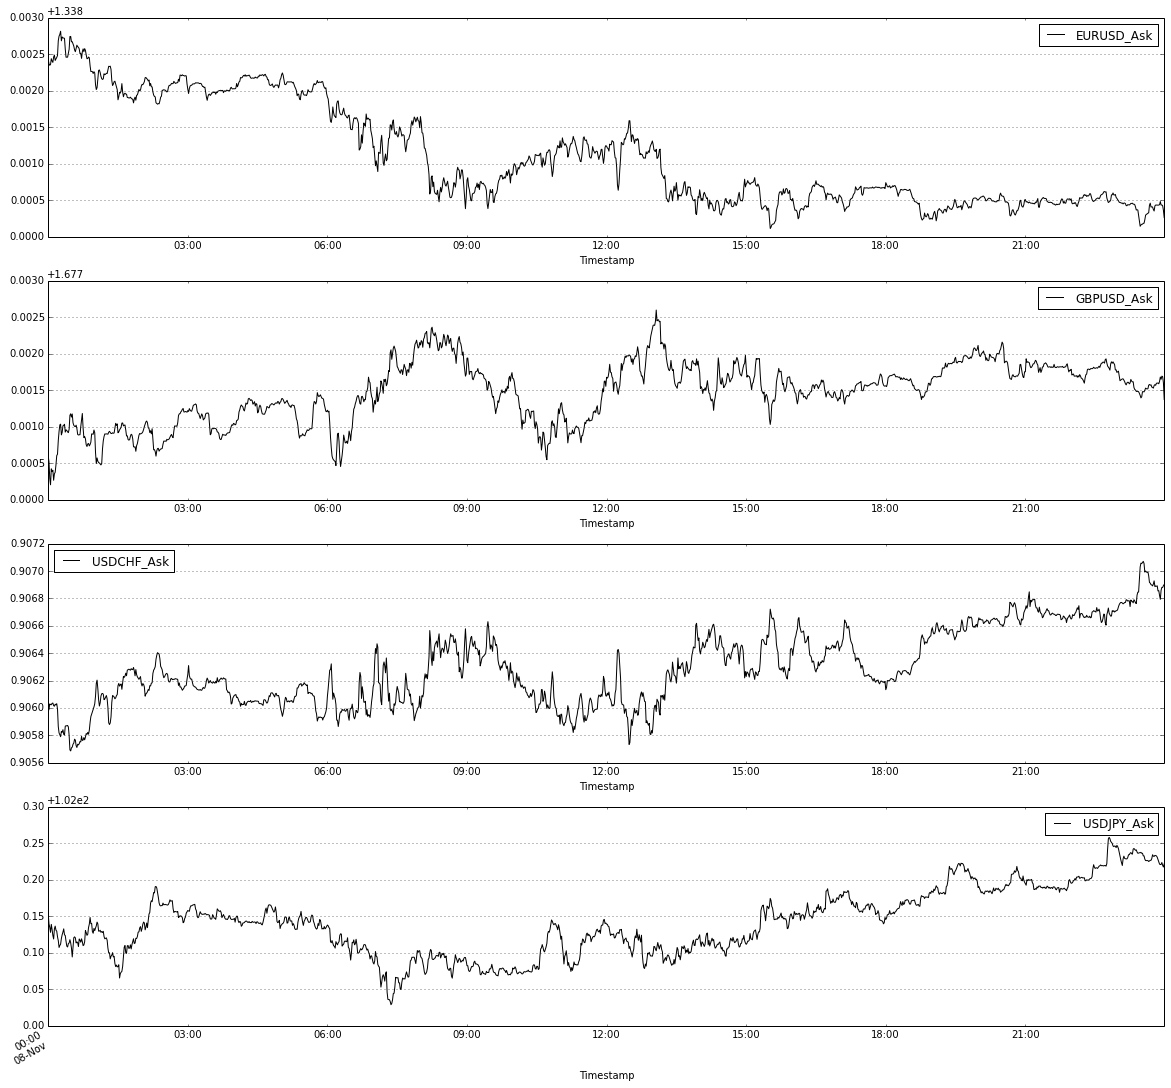
\includegraphics[width=\textwidth]{images/stocks_ask}
        \caption{Precio Ask de las divisas}
        \label{fig:stocks_ask}
    \end{center}
\end{figure}

Los ticks están compuestos por: \emph{Date}, \emph{Time}, \emph{Ask},
\emph{Bid}, \emph{AskVolume}, \emph{BidVolume}(ver tabla~\ref{tab:ticks}). Por
ser datos ticks, el campo Time es un hora \emph{double}, es decir, tiene
asociada una hora :minutos: segundos, donde segundos es un número no entero.
Cabe destacar que no existe una clara relación entre la aparición de ticks, ya
que en algunos casos aparecen hasta 4 ticks en 1 segundo, mientras que en otros
horarios no aparecen ticks en 90 segundos (dato calculado con la función
check\_min\_frequency de la clase Reader). En algunos casos, cómo en los días
más emblemáticos del año, que la cantidad de ticks por día incrementa
considerablemente, por ejemplo: un día reglar tiene aproximadamente 35 mil
ticks, mientras que días como 11 de Septiembre que hay 87 mil ticks. 

\begin{table}[h!]
\caption{Data Tick}
\label{tab:ticks}
\begin{center}
\begin{tabular}{|c|c|c|c|c|c|}
\hline
Date & Time & Ask & Bid& AskVolume & BidVolume \\
\hline
11-08-2014 & 00:00:00.000 & 1.34046 & 1.34042 & 1.25 & 1.69 \\
11-08-2014 & 00:00:02.159 & 1.34047 & 1.34043 & 4.69 & 1 \\
11-08-2014 & 00:00:02.667 & 1.34046 & 1.34042 & 1.32 & 2.44 \\
11-08-2014 & 00:00:03.175 & 1.34046 & 1.34043 & 1.32 & 1 \\
11-08-2014 & 00:00:07.058 & 1.34046 & 1.34043 & 3.75 & 1.69 \\
11-08-2014 & 00:00:07.362 & 1.34043 & 1.34041 & 2.25 & 1 \\
\hline
\end{tabular}
\end{center}
\end{table}
\newpage
En la figura \ref{fig:eurusd_ticks} se puede apreciar la data tick del EURUSD,
en una ventana de 30 minutos, donde la curva superior es la correspondiente al
Ask, y la inferior al Bid. En la figura \ref{fig:eurusd_freq} se muestra la
misma moneda pero con resamples a 1, 10, 30 y 60 segundos. El resample se
calcula con el promedio de los ticks en la ventana de 6 segundos, y para el
caso que no exista movimiento en dicho periodo, se rellena con el valor
anterior.

\begin{figure}[h!t]
    \begin{center}
        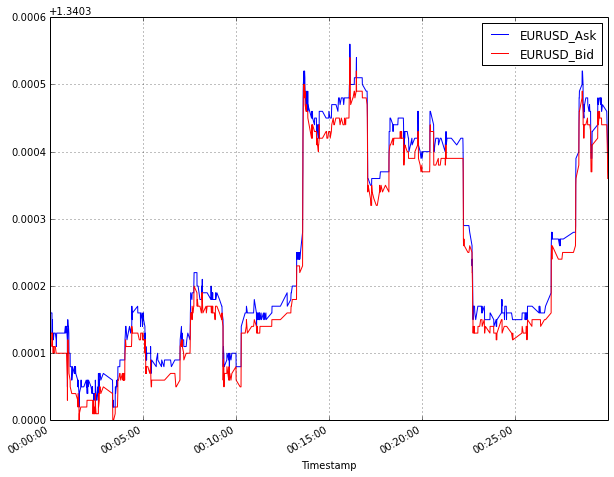
\includegraphics[width=0.7\textwidth]{images/eurusd}
        \caption{Ticks de EURUSD, Ventana de 30 minutos}
        \label{fig:eurusd_ticks}
    \end{center}
\end{figure}

\begin{figure}[h!t]
    \begin{center}
        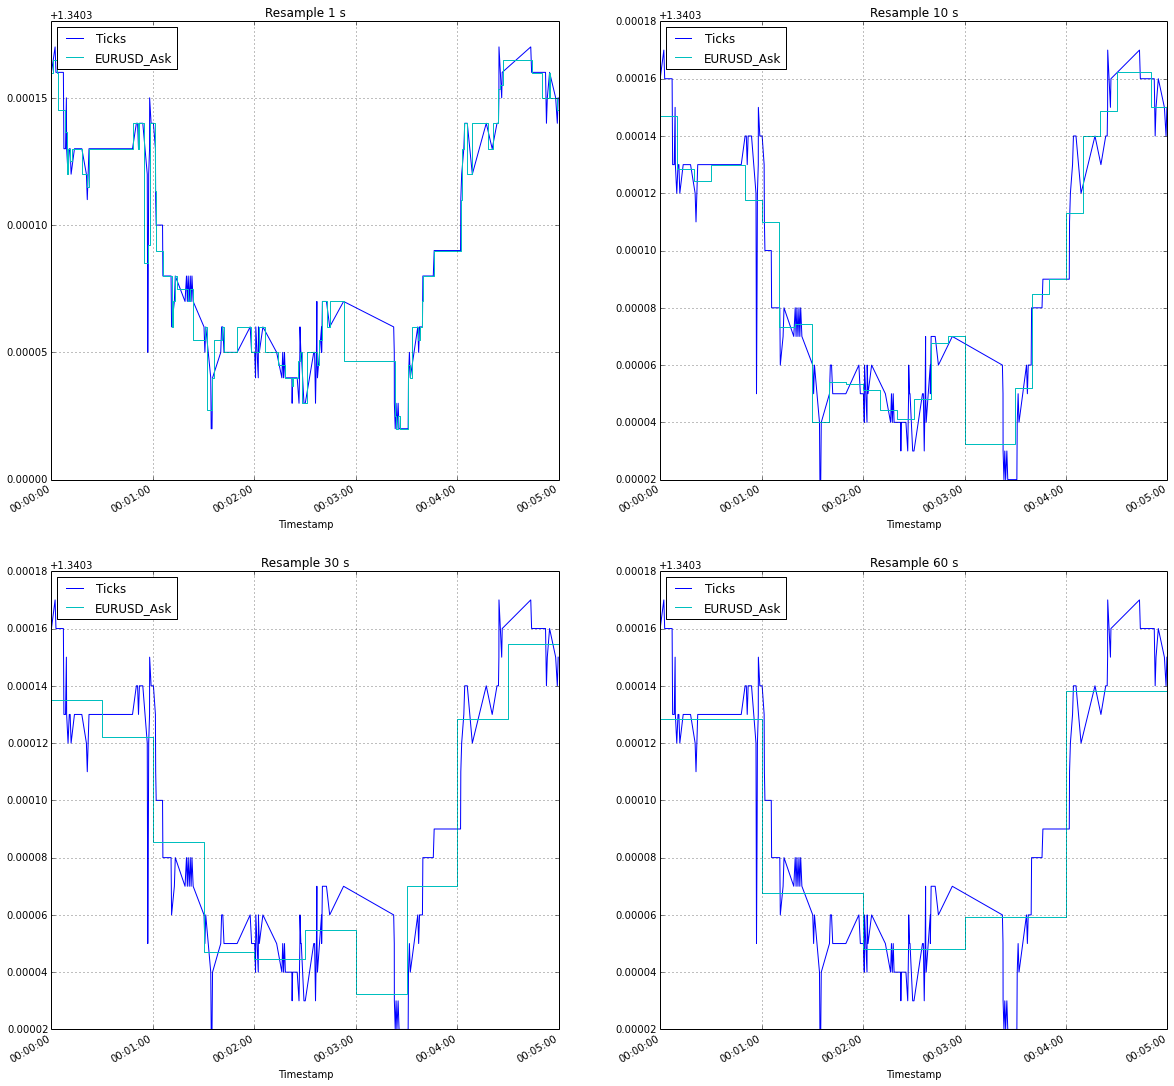
\includegraphics[width=\textwidth]{images/resample_freq}
        \caption{Ticks de EURUSD, Ventana de 30 minutos}
        \label{fig:eurusd_freq}
    \end{center}
\end{figure}

%\begin{figure}[h!t]
%    \begin{center}
%        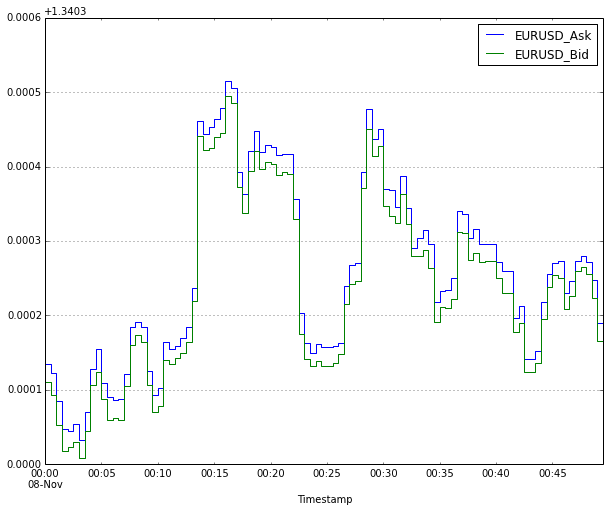
\includegraphics[width=0.6\textwidth]{images/eurusd_30s}
%        \caption{Ticks de EURUSD con resample de 30 segundos}
%        \label{fig:eurusd_30s}
%    \end{center}
%\end{figure}

\newpage
\section{Selección de Parámetros}
Cómo se mencionó anteriormente, los parámetros del algoritmo se calcularon
mediante el criterio de información de Akaike (AIC). Para esto, se tomaron
datos intra-diarios de agosto 2014, semana entre 11-15. Además, se
combinaron:
\begin{itemize}
 \item L: [100, 400, 700, 1000].
 \item P: [1, 2, 3, 4, 5].
 \item Frecuencias: 1 minuto.
\end{itemize}

Los resultados~\ref{tab:IAC} muestran para cada largo de ventana,
el número de lag óptimos (en negrita) para el modelo según el criterio de AIC.

\begin{table}[h]
\caption{Resultados de AIC}
\label{tab:IAC}
\begin{center}
\begin{tabular}{|l|c|c|c|c|c|}
\hline
\backslashbox{\textbf{L}}{\textbf{P}} & \textbf{1} & \textbf{2} & \textbf{3} & \textbf{4} & \textbf{5} \\
\hline
100 & -58.64574 & \textbf{-58.83743} & -58.70088 & -58.61984 & -58.68117 \\
400 & -60.42127 & -60.65667 & -60.67377 & -60.64634 &  \textbf{-60.68087} \\
700 & -59.05503 & -59.17413 & \textbf{-59.20871} & -59.18571 & -59.17367 \\
100 & -58.98121 & -59.09158 & \textbf{-59.12083} & -59.10099 & -59.0927 \\
\hline
\end{tabular}
\end{center}
\end{table}

\section{Pruebas de Cointegración}
Para los efectos de pruebas como se trabajó con 4 monedas, la cantidad de
vectores de cointegración debería ser 1, 2 o 3. 

\begin{figure}[h!t]
    \begin{center}
        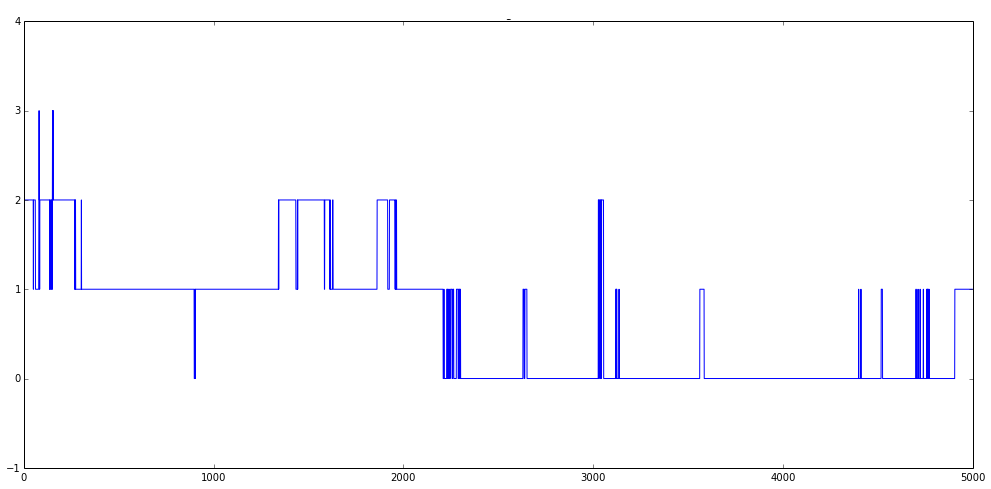
\includegraphics[width=0.6\textwidth]{images/betas}
        \caption{Pruebas de Cointegración}
        \label{fig:cointegracion}
    \end{center}
\end{figure}

Las pruebas de cointegración se realizaron al 95\% de significancia. Cómo se
puede observar, en algunos momentos la cantidad de vectores de cointegración no
son los esperados debido principalmente a la naturaleza y frecuencia de los
datos.

\section{Test de raíz unitaria}
Antes de correr los test, se checkearon que las series de tiempo fueran
I(1) usando el test de Augmented Dickey Fuller (ADF).

\begin{table}[h!]
\caption{Test de raíz unitaria, Frecuencia 60s}
\label{tab:adf_60s}
\begin{center}
\begin{tabular}{|l|c|c|c|c|c|}
\hline
& \textbf{Estadístico} & \textbf{Valor Crítico} & \textbf{Resultado}\\
\hline
EURUSD          & -0.64 & -1.94 & True       \\
$\Delta$ EURUSD & -70.45   & -1.94 & False       \\
GBPUSD          & -0.63   & -1.94 & True          \\
$\Delta$ GBPUSD & -54.53   & -1.94 & False       \\
CHFUSD          & -0.88   & -1.94 & True         \\
$\Delta$ CHFUSD & -98.98   & -1.94 & False       \\
JPYUSD          & -0.65 & -1.94 & True        \\
$\Delta$ JPYUSD & -85.78 & -1.94 & False     \\ 
\hline
\end{tabular}
\end{center}
\end{table}

\begin{table}[h!]
\caption{Test de raíz unitaria, Frecuencia 30s}
\label{tab:adf_30s}
\begin{center}
\begin{tabular}{|l|c|c|c|c|c|}
\hline
& \textbf{Estadístico} & \textbf{Valor Crítico} & \textbf{Resultado}\\
\hline
EURUSD          & -0.94 & -1.94 & True       \\
$\Delta$ EURUSD & -25.66   & -1.94 & False       \\
GBPUSD          & 0.29   & -1.94 & True          \\
$\Delta$ GBPUSD & -36.08   & -1.94 & False       \\
CHFUSD          & -0.49   & -1.94 & True         \\
$\Delta$ CHFUSD & -35.02   & -1.94 & False       \\
JPYUSD          & -0.45 & -1.94 & True        \\
$\Delta$ JPYUSD & -37.41 & -1.94 & False     \\ 
\hline
\end{tabular}
\end{center}
\end{table}

\begin{table}[h!]
\caption{Test de raíz unitaria, Frecuencia 10s}
\label{tab:adf_10s}
\begin{center}
\begin{tabular}{|l|c|c|c|c|c|}
\hline
& \textbf{Estadístico} & \textbf{Valor Crítico} & \textbf{Resultado}\\
\hline
EURUSD          & -0.85 & -1.94 & True       \\
$\Delta$ EURUSD & -43.91   & -1.94 & False       \\
GBPUSD          & 0.25   & -1.94 & True          \\
$\Delta$ GBPUSD & -40.81   & -1.94 & False       \\
CHFUSD          & -0.51   & -1.94 & True         \\
$\Delta$ CHFUSD & -61.12   & -1.94 & False       \\
JPYUSD          & -0.34 & -1.94 & True        \\
$\Delta$ JPYUSD & -46.38 & -1.94 & False     \\ 
\hline
\end{tabular}
\end{center}
\end{table}

Las tablas~\ref{tab:adf_60s}~\ref{tab:adf_30s}~\ref{tab:adf_60s} muestran que
todas las series no son rechazadas por el test de raíz unitaria pero si son
rechazadas para sus primeras diferencias (Con un valor crítico del 5\%). Esto
significa que todas las series de tiempo son I(1) por lo que es posible usar
los modelos VECM y OVECM. 

\section{Performance}
\subsection{Online VECM}
Dentro de todos los experimentos realizados, según la selección de parámetros
y considerando 400 iteraciones los resultados de tiempos de ejecución se pueden
ver en la tabla~\ref{tab:extimes}

\begin{table}[h!]
\caption{Tiempos de ejecución}
\label{tab:extimes}
\begin{center}
\begin{tabular}{|l|c|c|c|c|c|}
\hline
& L & P & e  & Tiempo[s] \\
\hline
OVECM & 100 &p=2  & 0      & 2.492\\
OVECM & 100 &p=2  & 0.0026  & 1.606\\
SLVECM & 100 &p=2& -- & 2.100\\
\hline
OVECM & 400 & p=5  & 0      & 3.513\\
OVECM & 400 &p=5  & 0.0041  & 2.569\\
SLVECM & 400 & p=5 & -- & 3.222\\
\hline
OVECM & 700 &p=3  & 0      & 3.296\\
OVECM & 700 &p=3  & 0.0032  & 2.856\\
SLVECM & 700 &p=3 & -- & 3.581\\
\hline
OVECM & 1000 & p=3 & 0      & 4.387\\
OVECM & 1000 & p=3  & 0.0022  & 2.408\\
SLVECM & 1000 & p=3  & -- & 3.609\\
\hline
\end{tabular}
\end{center}
\end{table}

OVECM recibe como parámetro el umbral de error para cambiar los vectores de
cointegración. Es decir, OVECM con e = 0 es lo mismo que ejecutar el SLVECM,
ambos tienen exactamente los mismos vectores de cointegración y estadísticos.

Para ver en detalle qué parte del código demora más se presenta el siguiente
profile de ejecución:
\begin{verbatim}
   Time %Time  Line Contents
============================
               def OVECM(y, L, P, it, avg_error, r, n):
      4   0.0      it2, l = y.shape
               
      7   0.0      dy_true = np.zeros([it, l], dtype=np.float32)
      4   0.0      dy_pred = np.zeros([it, l], dtype=np.float32)
      4   0.0      mape = np.zeros([it, l], dtype=np.float32)
      4   0.0      mae = np.zeros([it, l], dtype=np.float32)
      4   0.0      rmse = np.zeros([it, l], dtype=np.float32)
               
      8   0.0      m = cl.Matrix()
               
      3   0.0      start_time = time.time()
               
    911   0.0      for i in range(it):
 110712   1.6          y_i = y[i:i + L]
               
   1031   0.0          if i == 0:
                           # Initialization
   6839   0.1              beta = m.get_johansen(y_i.as_matrix(), 
                                    P, r)
  29075   0.4              A, B = m.vec_matrix(y_i, P, 
                                    beta.evecr)
                       else:
                           # Update & Out-of-sample forecast
4456245  66.1              A, B = m.vec_matrix_online(A, B, y_i, 
                                    P, beta.evecr)
   6820   0.1              dy_true[i-1, :] = B[-1,:]
  11775   0.2              dy_pred[i-1, :] = np.dot(A[-1,:], x)
               
                       # OLS
 439061   6.5          x, residuals, rank, s = np.linalg.lstsq(A, B)
  79004   1.2          Ax = np.dot(A, x)
               
                       # Internal mape
  28364   0.4          y_true = y_i.as_matrix()[-n:]
  23996   0.4          y_pred = Ax[-n:] + y_i.as_matrix()[-n - 1:-1]
               
                       # Stats info
 512572   7.6          stats = cl.stats(y_true, y_pred)
   8587   0.1          mape[i, :], mae[i,:], rmse[i,:] = stats.mape, 
                            stats.mae, stats.rmse
  36757   0.5          avg_mape = np.average(mape[i, :])
               
                       # Beta update
   2224   0.0          if avg_mape > avg_error:
 865051  12.8              beta = m.get_johansen(y_i.as_matrix(), P)
    307   0.0              r = beta.r
  41151   0.6              A = m.vec_matrix_update(A, y_i, P, 
                                beta.evecr)
  79857   1.2              x, residuals, rank, s = np.linalg.lstsq(A, B)
               
                   # model_it object
   2945   0.0      oecm = cl.model_it(y[L:L + it], dy_pred + 
                        y[L - 1:L + it - 1], dy_true, dy_pred, 
                        mape, mae, rmse)


 Time  Per Hit   % Time  Line Contents
======================================
                         @do_profile(follow=[OVECM, OVECMRR])
                         def main():
    2      2.0      0.0      path = '../data_csv/data_ticks/august_11/'
    2      2.0      0.0      assets = ['EURUSD', 'GBPUSD', 
                                    'USDCHF', 'USDJPY']
                             
    6      1.2      0.0      data_list = [path+ i +'.csv' for i in assets]
                             
    7      7.0      0.0      reader = cl.Reader(data_list)
 100M   100M.0     93.7      ticks_list = reader.load()
                         
39925  39925.0      0.0      ask_norm = reader.resample_list(ticks_list, 
                            '60s', [2, 3])            
    2      2.0      0.0      y = ask_norm
                         
    1      1.0      0.0      L = 1000
    1      1.0      0.0      P = 4
    1      1.0      0.0      it = 400
    1      1.0      0.0      r = 0
    0      0.0      0.0      n = 50
    1      1.0      0.0      avg_error = 0.002
                         
 6758K 6758K.0      6.3      oecm = OVECM(y, L, P, it, avg_error, r, n)

\end{verbatim}

Se puede observar que los cálculos más costosos son la construcción de la
matriz VECM, seguido por el cálculo de los vectores de cointegración, luego de
los estadísticos en cada paso y finalmente la resolución del sistema mediante
mínimos cuadrados. Por otro lado, el cálculo está inserto dentro de la lectura
de archivos, los cuales toman mucho más tiempo que la ejecución del algoritmo.

Cabe destacar que estos números dependen del tamaño de la ventana, número de
lags, umbral de error y cantidad de elementos para calcular el mape in-sample.

En todos los casos, ya sea incluso en frecuencias de 1 segundo, el algoritmo
OVECM, toma tiempos de ejecución menor a la frecuencia de datos, esto le
permite a un algoritmo de estrategia poder utilizar como entrada los resultados
de esta implementación.

\subsection{Algoritmo de Coleman GPU}
Como una alternativa a mínimos cuadrados clásico, se implementó una versión
serial y paralela usando scikits.cuda del algoritmo propuesto en
\cite{coleman2010}. Para correr las pruebas es necesario configurar una
serie de paquetes y bibliotecas, por lo que las pruebas se hicieron de forma
local, usando una tarjeta nvidia GTX 760. 

Las pruebas se realizaron con datos generados mediante la función randomMatrix
de la clase Matrix, en donde se puede configurar el tamaño de matriz y el rank
de la matriz. Los resultados para casos reales no son alentadores (sistema de
ecuaciones $Ax = b$ donde A tiene muchas filas y pocas columnas), se puede ver
en la tabla~\ref{fig:speedup_real}, que CPU demora aproximadamente un tercio de
GPU, diferencia que disminuye en cuanto la cantidad de filas aumente.

EL mismo algoritmo fue comparado para casos donde las matrices son cuadradas de
gran dimensión. Se puede observar en la figura~\ref{fig:speedup_square} que en
estos casos si GPU tiene mejor performance que CPU.

\begin{figure}[h!t]
    \begin{center}
        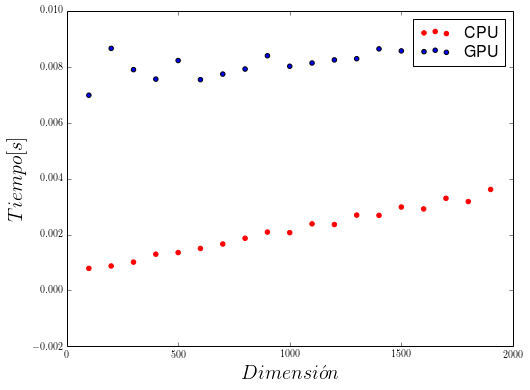
\includegraphics[width=0.7\textwidth]{images/speed_up_real}
        \caption{Comparación tiempos de ejecución CPU y GPU, modelo real}
        \label{fig:speedup_real}
    \end{center}
\end{figure}

\begin{figure}[h!t]
    \begin{center}
        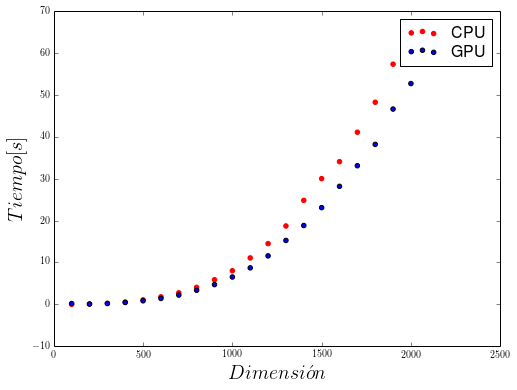
\includegraphics[width=0.7\textwidth]{images/speed_up_square}
        \caption{Comparación tiempos de ejecución CPU y GPU, matrices cuadradas}
        \label{fig:speedup_square}
    \end{center}
\end{figure}

\section{Resultados}
Uno de los objetivos del algoritmo OVECM es ser más eficiente en tiempo que el
SLVECM, pero además se busca que los errores de la extrapolación no sean tan
distintos. La tabla~\ref{tab:mapes_60s}~\ref{tab:mapes_30s}~\ref{tab:mapes_10s}
muestran los diferentes indicadores de las muestras en la interpolación
(in-sample) y la extrapolación (out-of-sample). Se puede ver que son similares,
por lo que se confirma que los vectores de cointegración se pueden mantener en
cierta medida durante el tiempo. Es importante notar además que a medida que
aumenta la frecuencia, los indicadores son menores, ya que la alta frecuencia
refleja menores fluctuaciones en los valores de las divisas.

\begin{table*}[ht!]
\caption{Métricas del modelo, Frecuencia 60s}
\label{tab:mapes_60s}
\begin{center}
\begin{adjustbox}{max width=\textwidth}
\begin{tabular}{|l|l|c|c|c|c|c|c|c|c|}
\hline
\multicolumn{4}{|c|}{Model} & \multicolumn{3}{|c|}{In-sample} &
\multicolumn{3}{|c|}{Out-of-sample} \\ 
\hline
\hline
Método & L & P & e &
MAPE & MAE& RMSE&
MAPE & MAE& RMSE \\
\hline
 OVECM  &   100  &  P=2& 0.0026  &  0.00263&  0.00085&  0.00114&  0.00309&  0.00094&  0.00131\\
 OVECM  &   400  &  P=5& 0.0041  &  0.00378&  0.00095&  0.00127&  0.00419&  0.00103&  0.00143\\
 OVECM  &   700  &  P=3& 0.0032  &  0.00323&  0.00099&  0.00130&  0.00322&  0.00097&  0.00132\\
 OVECM  &   1000 &  P=3& 0.0022  &
 \textbf{0.00175}&  \textbf{0.00062}&  \textbf{0.00087} &
 \textbf{0.00172}&  \textbf{0.00061}&  \textbf{0.00090}\\
\hline
 SLVECM  &   100 &  P=2& -  &  0.00262&  0.00085&  0.00113&  0.00310&  0.00095&  0.00132\\
 SLVECM  &   400 &  P=5& -  &  0.00375&  0.00095&  0.00126&  0.00419&  0.00103&  0.00143\\
 SLVECM  &   700 &  P=3& -  &  0.00324&  0.00099&  0.00130&  0.00322&  0.00098&  0.00132\\
 SLVECM  &   1000 &  P=3& -  &
 \textbf{0.00174}&  \textbf{0.00061}&  \textbf{0.00087}&
 \textbf{0.00172}&  \textbf{0.00061}&  \textbf{0.00090}\\
\hline
\end{tabular}
\end{adjustbox}
\end{center}
\end{table*}

\begin{table*}[ht!]
\caption{Métricas del modelo, Frecuencia 30s}
\label{tab:mapes_30s}
\begin{center}
\begin{adjustbox}{max width=\textwidth}
\begin{tabular}{|l|l|c|c|c|c|c|c|c|c|}
\hline
\multicolumn{4}{|c|}{Model} & \multicolumn{3}{|c|}{In-sample} &
\multicolumn{3}{|c|}{Out-of-sample} \\ 
\hline
\hline
Método & L & P & e &
MAPE & MAE& RMSE&
MAPE & MAE& RMSE \\
\hline
 OVECM  &   100  &  P=2 &  0.0015  &  0.00156  &  0.00056  &  0.00077  &  0.00180  &  0.00067  &  0.00095 \\
 OVECM  &   400  &  P=5 &  0.0014  &  0.00140  &  0.00050  &  0.00070  &  0.00162  &  0.00059  &  0.00085 \\
 OVECM  &   700  &  P=3 &  0.0028  &  0.00287  &  0.00078  &  0.00105  &  0.00309  &  0.00081  &  0.00112 \\
 OVECM  &   1000 &  P=3 &  0.0024  &  \textbf{0.00245}  &  \textbf{0.00058}  &  \textbf{0.00079}  &  \textbf{0.00239}
   &  \textbf{0.00057}  &  \textbf{0.00082} \\
\hline
 SLVECM  &   100 &  P=2& -  &  0.00156  &  0.00056  &  0.00077  &  0.00176  &  0.00066  &  0.00095 \\
 SLVECM  &   400 &  P=5& -  &  0.00140  &  0.00050  &  0.00069  &  0.00162  &  0.00058  &  0.00085 \\
 SLVECM  &   700 &  P=3& -  &  0.00287  &  0.00077  &  0.00105  &  0.00308  &  0.00081  &  0.00111 \\
 SLVECM  &   1000&  P=3& -  &  \textbf{0.00245}  &  \textbf{0.00058}  &  \textbf{0.00079}  &  
  \textbf{0.00239}  &  \textbf{0.00057}  &  \textbf{0.00082} \\
\hline
\end{tabular}
\end{adjustbox}
\end{center}
\end{table*}

\begin{table*}[ht!]
\caption{Métricas del modelo, Frecuencia 10s}
\label{tab:mapes_10s}
\begin{center}
\begin{adjustbox}{max width=\textwidth}
\begin{tabular}{|l|l|c|c|c|c|c|c|c|c|}
\hline
\multicolumn{4}{|c|}{Model} & \multicolumn{3}{|c|}{In-sample} &
\multicolumn{3}{|c|}{Out-of-sample} \\ 
\hline
\hline
Método & L & P & e &
MAPE & MAE& RMSE&
MAPE & MAE& RMSE \\
\hline
 OVECM  &   100  &  P=2 &  0.0012  &  0.00124  &  0.00047  &  0.00065  &  0.00135  &  0.00052  &  0.00073 \\
 OVECM  &   400  &  P=5 &  0.0010  &  0.00108  &  0.00043  &  0.00061  &  0.00113  &  0.00047  &  0.00067 \\
 OVECM  &   700  &  P=3 &  0.0008  &  0.00085  &  0.00031  &  0.00045  &  0.00086  &  0.00032  &  0.00048 \\
 OVECM  &   1000 &  P=3 &  \textbf{0.0062}  &  \textbf{0.00062}  &  \textbf{0.00020}  &  \textbf{0.00033}  &  
      \textbf{0.00062}  &  \textbf{0.00020}  &  \textbf{0.00033} \\
\hline
 SLVECM  &   100 &  P=2 & -  &  0.00124  &  0.00047  &  0.00065  &  0.00136  &  0.00052  &  0.00073 \\
 SLVECM  &   400 &  P=5 & -  &  0.00108  &  0.00043  &  0.00061  &  0.00113  &  0.00047  &  0.00067 \\
 SLVECM  &   700 &  P=3 & -  &  0.00084  &  0.00031  &  0.00045  &  0.00086  &  0.00032  &  0.00048 \\
 SLVECM  &   1000 &  P=3& -  &  \textbf{0.00063}  &  \textbf{0.00020}  &  \textbf{0.00033}  &  
      \textbf{0.00063}  &  \textbf{0.00020}  &  \textbf{0.00033} \\
\hline
\end{tabular}
\end{adjustbox}
\end{center}
\end{table*}

En la figura~\ref{fig:accuracy} se puede observar qué tan bien aproxima el
método OVECM para cada divisa. En la figura~\ref{fig:mapes} se puede observar
cuánto es el error de aproximación medido en MAPE in-sample para cada iteración.

\begin{figure}[h!t]
    \begin{center}
        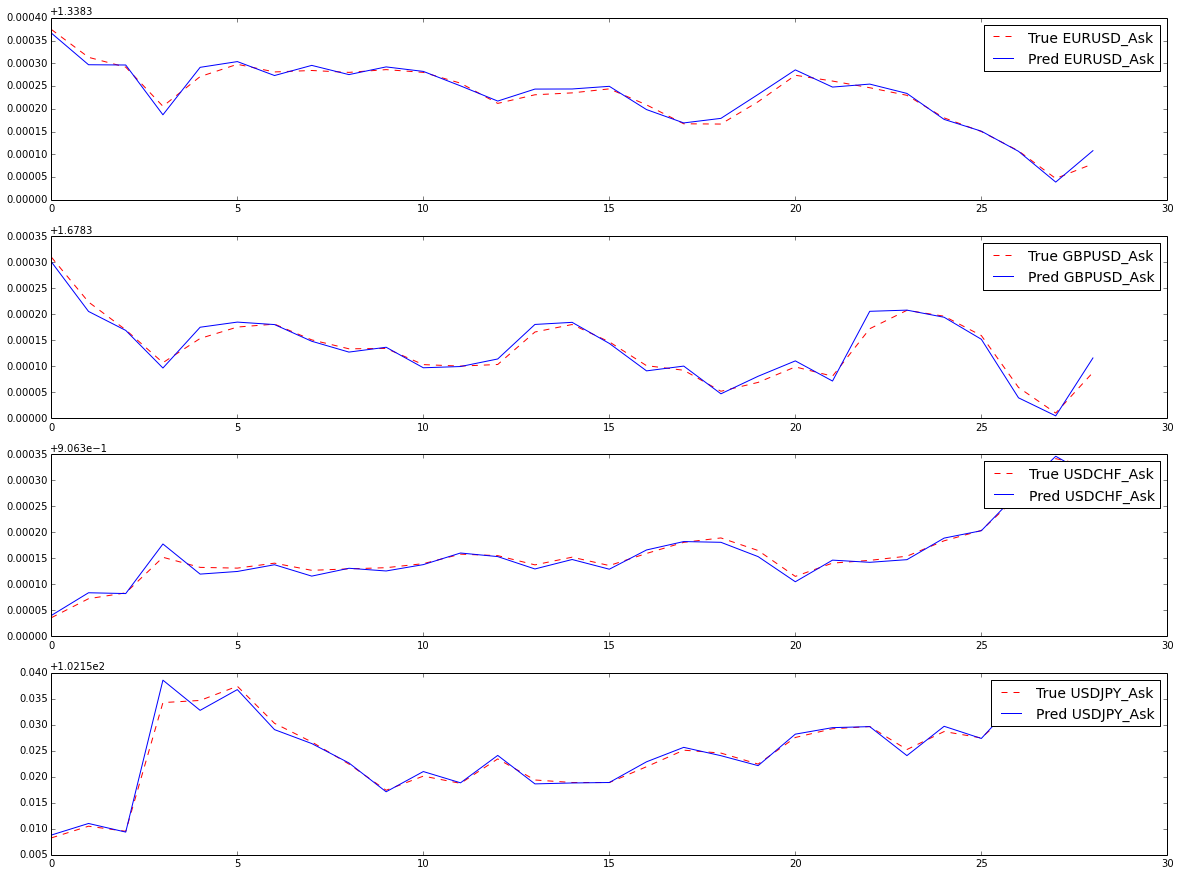
\includegraphics[width=\textwidth]{images/y_vs_yhat}
        \caption{Divisas: Valor real y aproximación}
        \label{fig:accuracy}
    \end{center}
\end{figure}


\begin{figure}[h!t]
    \begin{center}
        %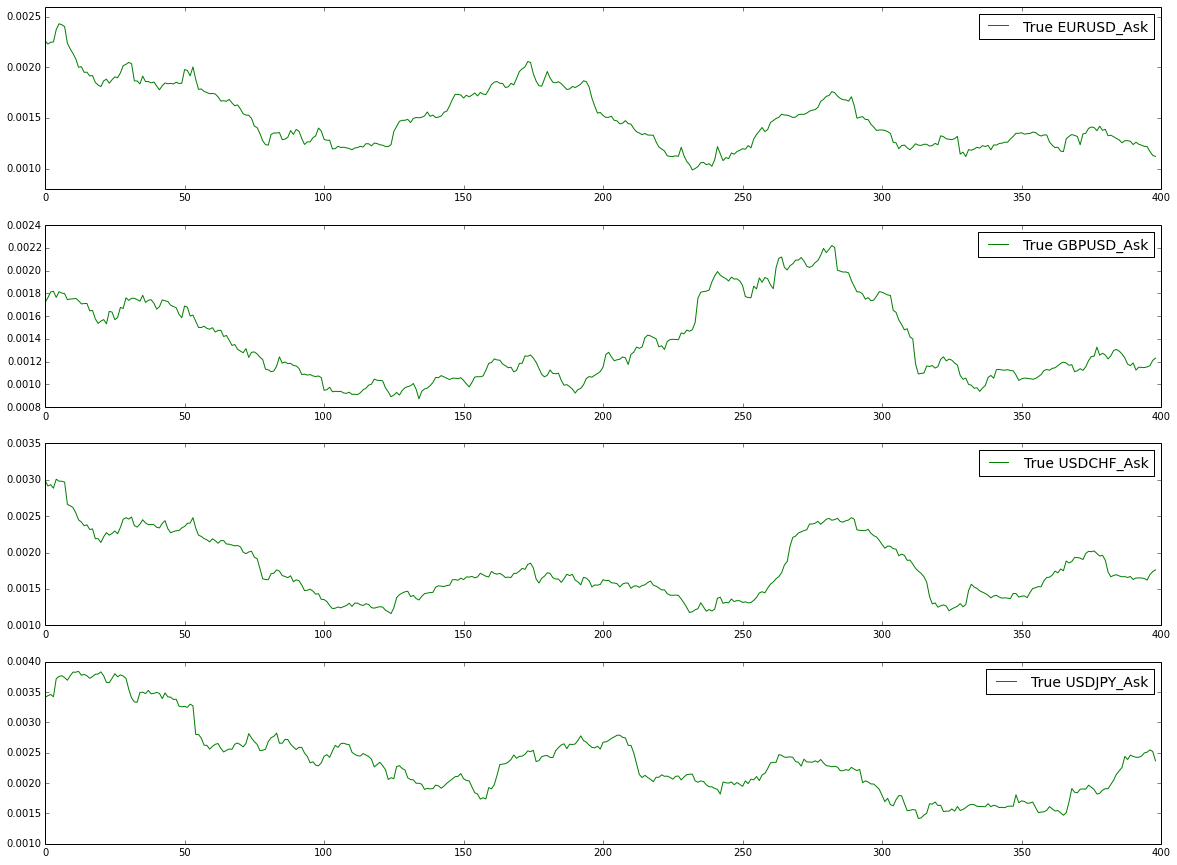
\includegraphics[width=\textwidth]{images/ovecm_mapes}
        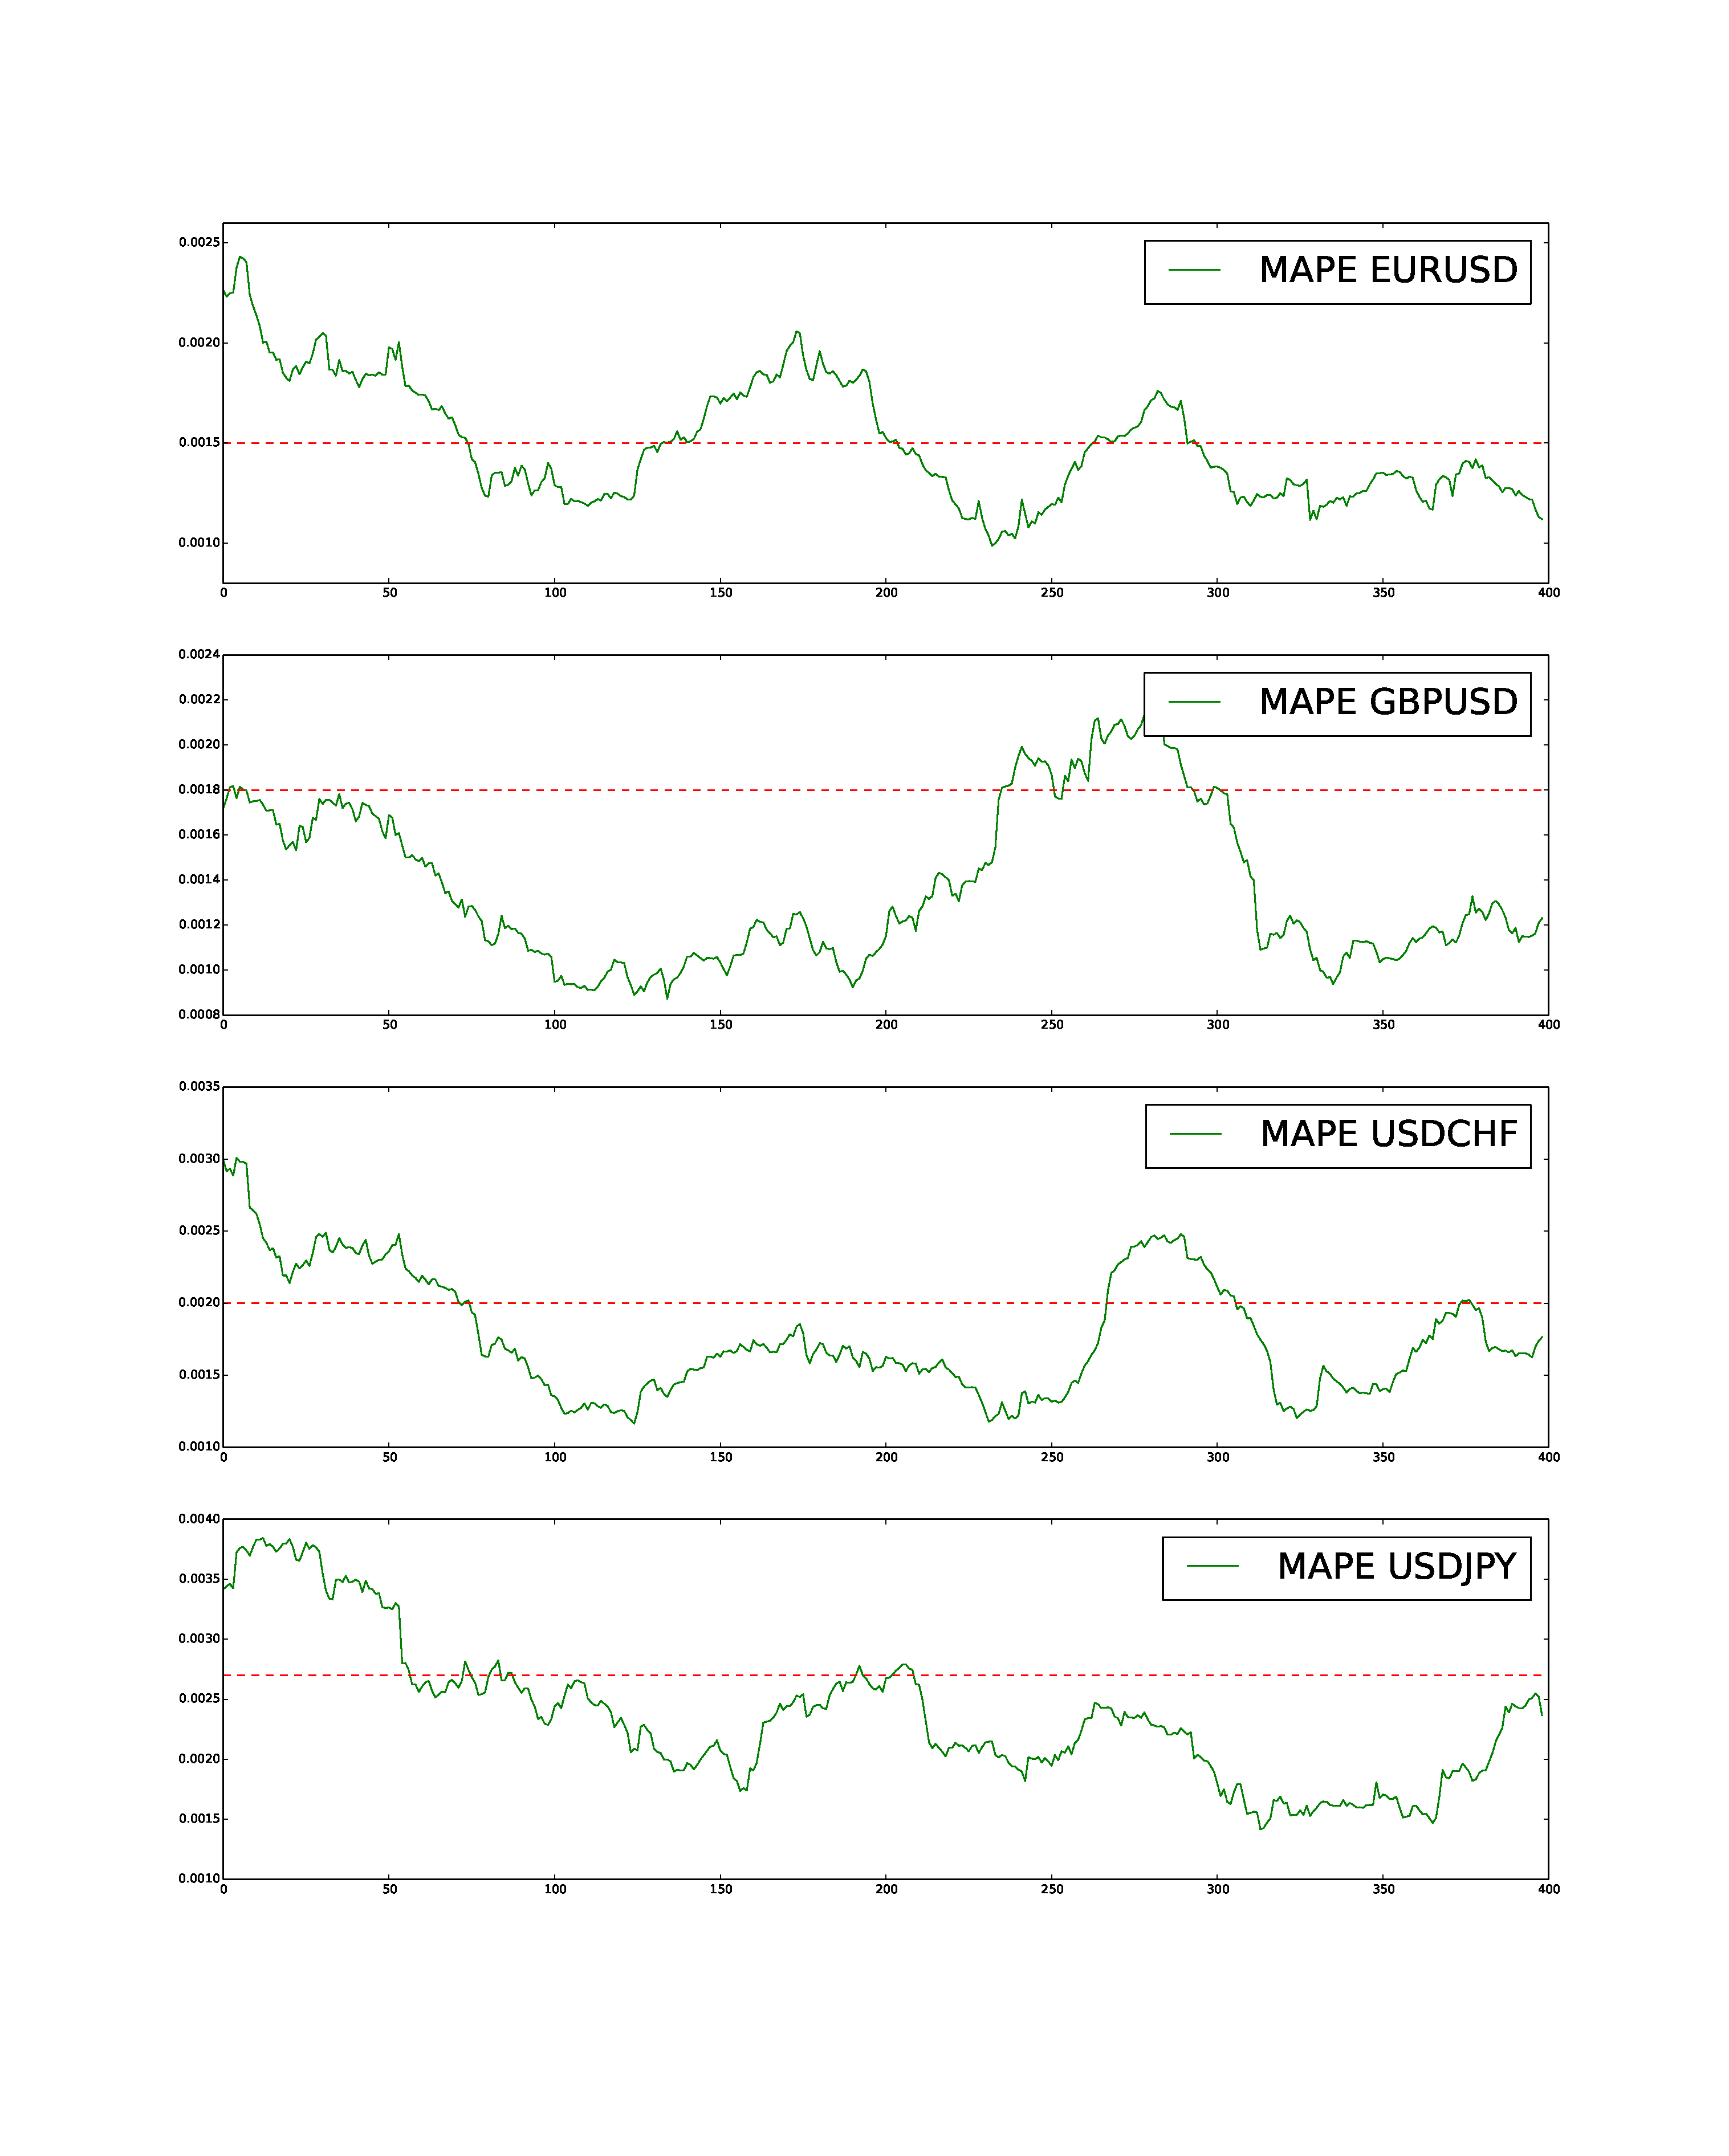
\includegraphics[width=\textwidth]{images/mapes}
        \caption{Divisas: Valor del MAPE en cada iteración}
        \label{fig:mapes}
    \end{center}
\end{figure}
